\documentclass[../mathNotesPreamble]{subfiles}
\begin{document}
%  \relscale{1.4}
  \section{6.6: Surface Area}

  \begin{defn*}[Area of a Surface of Revolution]
    Let $f$ be a nonnegative function with a continuous first derivative on the interval $\sbrkt{a,b}$. The area of the surface generated when the graph of $f$ on the interval $\sbrkt{a,b}$ is revolved around the $x$-axis is
      \[S=\int_a^b 2\pi f(x)\sqrt{1+f'(x)^2}\,dx.\]
  \end{defn*}

  \begin{center}
    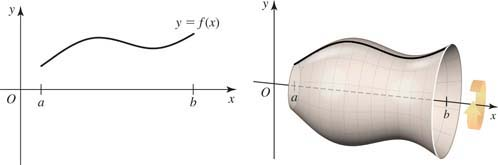
\includegraphics[width=0.5\linewidth]{../images/briggs_06_06/fig06_60}
  \end{center}

  \begin{ex*}
    Find the exact area of the surface obtained by rotating the curve $y=x^3$, $0\leq x\leq 2$ about the $x$-axis.
  \end{ex*}
  \vspace*{\stretch{1}}
  \pagebreak

  \begin{ex*}
    Find the exact area of the surface obtained by rotating the curve $y=\sqrt{8x-x^2}$, $1\leq x\leq 7$ about the $x$-axis.
  \end{ex*}
  \vspace*{\stretch{1}}
  \pagebreak

  \begin{ex*}
    Find the exact area of the surface obtained by rotating the curve $y=\dfrac{1}{2}\parens{e^{x}+e^{-x}}$, $-\ln(2)\leq x\leq \ln(2)$ about the $x$-axis.
  \end{ex*}
  \vspace*{\stretch{1}}
  \pagebreak

  

\end{document}
